\documentclass{article}
\usepackage{graphicx, tikz-cd, float, titlepic, booktabs} % Required for inserting images
\usepackage{pgfplots}
\pgfplotsset{compat=1.15}
\usepackage{mathrsfs}
\usetikzlibrary{arrows}
\usepackage{amsmath, amssymb, amsthm, amsfonts, siunitx, physics, gensymb}
\AtBeginDocument{\RenewCommandCopy\qty\SI}
\usepackage[version=4]{mhchem}
\usepackage[most,many,breakable]{tcolorbox}
\usepackage{xcolor, fancyhdr, varwidth}
\usepackage[Glenn]{fncychap}
%Options: Sonny, Lenny, Glenn, Conny, Rejne, Bjarne, Bjornstrup
\usepackage{hyperref, cleveref}
\usepackage{icomma, enumitem} %comma as decimal and continue enumerate with [resume]
\usepackage[danish]{babel}
%%%%%%%%%%%%%%%%%%%%%%%%%%%%%%
% SELF MADE COLORS
%%%%%%%%%%%%%%%%%%%%%%%%%%%%%%
\definecolor{myg}{RGB}{56, 140, 70}
\definecolor{myb}{RGB}{45, 111, 177}
\definecolor{myr}{RGB}{199, 68, 64}
\definecolor{mytheorembg}{HTML}{F2F2F9}
\definecolor{mytheoremfr}{HTML}{00007B}
\definecolor{mylenmabg}{HTML}{FFFAF8}
\definecolor{mylenmafr}{HTML}{983b0f}
\definecolor{mypropbg}{HTML}{f2fbfc}
\definecolor{mypropfr}{HTML}{191971}
\definecolor{myexamplebg}{HTML}{F2FBF8}
\definecolor{myexamplefr}{HTML}{88D6D1}
\definecolor{myexampleti}{HTML}{2A7F7F}
\definecolor{mydefinitbg}{HTML}{E5E5FF}
\definecolor{mydefinitfr}{HTML}{3F3FA3}
\definecolor{notesgreen}{RGB}{0,162,0}
\definecolor{myp}{RGB}{197, 92, 212}
\definecolor{mygr}{HTML}{2C3338}
\definecolor{myred}{RGB}{127,0,0}
\definecolor{myyellow}{RGB}{169,121,69}
\definecolor{myexercisebg}{HTML}{F2FBF8}
\definecolor{myexercisefg}{HTML}{88D6D1}
%%%%%%%%%%%%%%%%%%%%%%%%%%%%%%%%%%%%%%%%%%%%%%%%%%%%%%%%%%%%%%%%%%%%%%
% Box environments for theorems and problems
%%%%%%%%%%%%%%%%%%%%%%%%%%%%%%%%%%%%%%%%%%%%%%%%%%%%%%%%%%%%%%%%%%%%%
\setlength{\parindent}{1cm}
%================================
% Question BOX
%================================
\makeatletter
\newtcbtheorem{question}{Opgave}{enhanced,
	breakable,
	colback=white,
	colframe=myb!80!black,
	attach boxed title to top left={yshift*=-\tcboxedtitleheight},
	fonttitle=\bfseries,
	title={#2},
	boxed title size=title,
	boxed title style={%
			sharp corners,
			rounded corners=northwest,
			colback=tcbcolframe,
			boxrule=0pt,
		},
	underlay boxed title={%
			\path[fill=tcbcolframe] (title.south west)--(title.south east)
			to[out=0, in=180] ([xshift=5mm]title.east)--
			(title.center-|frame.east)
			[rounded corners=\kvtcb@arc] |-
			(frame.north) -| cycle;
		},
	#1
}{def}
\makeatother
%================================
% DEFINITION BOX
%================================

\newtcbtheorem[]{Definition}{Definition}{enhanced,
	before skip=2mm,after skip=2mm, colback=red!5,colframe=red!80!black,boxrule=0.5mm,
	attach boxed title to top left={xshift=1cm,yshift*=1mm-\tcboxedtitleheight}, varwidth boxed title*=-3cm,
	boxed title style={frame code={
					\path[fill=tcbcolback]
					([yshift=-1mm,xshift=-1mm]frame.north west)
					arc[start angle=0,end angle=180,radius=1mm]
					([yshift=-1mm,xshift=1mm]frame.north east)
					arc[start angle=180,end angle=0,radius=1mm];
					\path[left color=tcbcolback!60!black,right color=tcbcolback!60!black,
						middle color=tcbcolback!80!black]
					([xshift=-2mm]frame.north west) -- ([xshift=2mm]frame.north east)
					[rounded corners=1mm]-- ([xshift=1mm,yshift=-1mm]frame.north east)
					-- (frame.south east) -- (frame.south west)
					-- ([xshift=-1mm,yshift=-1mm]frame.north west)
					[sharp corners]-- cycle;
				},interior engine=empty,
		},
	fonttitle=\bfseries,
	title={#2},#1}{def}
\newtcbtheorem[]{definition}{Definition}{enhanced,
	before skip=2mm,after skip=2mm, colback=red!5,colframe=red!80!black,boxrule=0.5mm,
	attach boxed title to top left={xshift=1cm,yshift*=1mm-\tcboxedtitleheight}, varwidth boxed title*=-3cm,
	boxed title style={frame code={
					\path[fill=tcbcolback]
					([yshift=-1mm,xshift=-1mm]frame.north west)
					arc[start angle=0,end angle=180,radius=1mm]
					([yshift=-1mm,xshift=1mm]frame.north east)
					arc[start angle=180,end angle=0,radius=1mm];
					\path[left color=tcbcolback!60!black,right color=tcbcolback!60!black,
						middle color=tcbcolback!80!black]
					([xshift=-2mm]frame.north west) -- ([xshift=2mm]frame.north east)
					[rounded corners=1mm]-- ([xshift=1mm,yshift=-1mm]frame.north east)
					-- (frame.south east) -- (frame.south west)
					-- ([xshift=-1mm,yshift=-1mm]frame.north west)
					[sharp corners]-- cycle;
				},interior engine=empty,
		},
	fonttitle=\bfseries,
	title={#2},#1}{def}

\newtcbtheorem{theo}%
    {Theorem}{}{theorem}
\newtcolorbox{prob}[1]{colback=red!5!white,colframe=red!50!black,fonttitle=\bfseries,title={#1}}
%================================
% NOTE BOX
%================================

\usetikzlibrary{arrows,calc,shadows.blur}
\tcbuselibrary{skins}
\newtcolorbox{note}[1][]{%
	enhanced jigsaw,
	colback=gray!20!white,%
	colframe=gray!80!black,
	size=small,
	boxrule=1pt,
	title=\textbf{Note:},
	halign title=flush center,
	coltitle=black,
	breakable,
	drop shadow=black!50!white,
	attach boxed title to top left={xshift=1cm,yshift=-\tcboxedtitleheight/2,yshifttext=-\tcboxedtitleheight/2},
	minipage boxed title=1.5cm,
	boxed title style={%
			colback=white,
			size=fbox,
			boxrule=1pt,
			boxsep=2pt,
			underlay={%
					\coordinate (dotA) at ($(interior.west) + (-0.5pt,0)$);
					\coordinate (dotB) at ($(interior.east) + (0.5pt,0)$);
					\begin{scope}
						\clip (interior.north west) rectangle ([xshift=3ex]interior.east);
						\filldraw [white, blur shadow={shadow opacity=60, shadow yshift=-.75ex}, rounded corners=2pt] (interior.north west) rectangle (interior.south east);
					\end{scope}
					\begin{scope}[gray!80!black]
						\fill (dotA) circle (2pt);
						\fill (dotB) circle (2pt);
					\end{scope}
				},
		},
	#1,
}

%%%%%%%%%%%%%%%%%%%%%%%%%%%%%%%%%%%%%%%%%%%%%%%%%%%%%%%%%%%%%%%%%
% SELF MADE COMMANDS
%%%%%%%%%%%%%%%%%%%%%%%%%%%%%%
\newcommand{\sol}{\setlength{\parindent}{0cm}\textbf{\textit{Løsning:}}\setlength{\parindent}{1cm}}
%%%%%%%%%%%%%%%%%%%%%%%%%%%%%%%%%
\usepackage[tmargin=2cm,rmargin=1in,lmargin=1in,margin=0.85in,bmargin=2cm,footskip=.2in]{geometry}\pagestyle{fancy}
\lhead{Minrui Kevin Zhou 2.b}
\rhead{Aflevering 26}

\title{Aflevering 26\\
{\Large \textbf{2.b mat A}}}
\author{Kevin Zhou}
\date{\today}

\begin{document}
\maketitle
\section*{Bedømmelseskriterier:}
\begin{itemize}
    \setlength\itemsep{3cm}
    \Large
    \item  Redegørelse og dokumentation for metode
    \item Figurer, grafer og andre illustrationer
    \item Notation og layout
    \item Formidling og forklaring
\end{itemize}
\pagebreak
\begin{question}{}{}
  En linje $l$ er givet ved ligningen
  \[
  5 \cdot \left(x-7\right) +4 \cdot \left(y-2\right) =0
  \] 
  \begin{itemize}
    \item[a.] Angiv en normalvektor til linjen $l$.
    \item[b.] Angiv et punkt $P_0$ på linjen $l$. 
  \end{itemize}
\end{question}
\sol \\
\textbf{a.}
Fra linjens ligning ses det, at en normalvektor til linjen må være
\[
\va{n} =\mqty(5\\ 4) 
\] 
\textbf{b.}
Lad $P_0$ have $x$-værdien 7. 
Så kan vi regne $y$-værdien for punktet, da det må opfylde linjens ligning.
\begin{equation*}
\begin{split}
  5 \cdot \left(x-7\right) +4 \cdot \left(y-2\right) =0 &\iff 4 \cdot \left(y-2\right) =0 \\ 
  &\iff y=2
\end{split}
\end{equation*}
Altså har vi
\[
P_0=(7,2)
\] 
\begin{question}{}{}
  En linje $l$ har parameterfremstillingen
  \[
  l: \mqty(x\\ y) =\mqty(1\\ 3) + t \cdot \mqty(2\\ 1), \quad t \in \mathbb{R}
  \] 
  Bestem en ligning for den linje $m$, der går gennem punktet $(3,4)$ og er vinkelret på $l$.
\end{question}
\sol \\
Vektoren $\mqty(2\\ 1) $ er en retningsvektor for $l$.
Derfor kan den da være en normalvektor til linjen $m$.
Da $m$ skal gå gennem $(3,4)$, så kan en ligning for $m$ være 
\[
2 \cdot \left(x-3\right) + 1 \cdot \left(y-4\right) =0 \iff 2x+y-10=0
\] 
\begin{question}{}{}
  To linjer i planen er givet ved ligningerne
  \begin{equation*}
  \begin{split}
    &l: x-2y-5=0 \\
    &m: -3x +6y+12=0
  \end{split}
  \end{equation*}
  \begin{itemize}
    \item[a.] Gør rede for, at de to linjer er parallelle.
    \item[b.] Bestem afstanden mellem de to linjer.
  \end{itemize}
\end{question}
\sol \\
\textbf{a.}
Vi kan fra ligningerne se, at en normalvektor for $l$ er $\mqty(1\\ -2) $ og en normalvektor for $m$ er $\mqty(-3\\ 6) $. 
Siden der gælder, at
\[
-2 \cdot \mqty(1\\ -2) =\mqty(-3\\ 6) 
\] 
så er de to normalvektorer for $l$ og $m$ skalare multipla, hvilket medfører, at de to normalvektorer er parallele. 
Da to normalvektorer for $m$ og $l$ er parallele, så må $m$ og $l$ også være parallele. \\[1ex]
\textbf{b.} 
Afstanden mellem de to linjer må være afstanden mellem et punkt, der tilhører den ene linje, og den anden linje.
Vi ser da, at $P_0=(1,-\frac{3}{2})\in m$. Vi har da
\begin{equation*}
\begin{split}
  \text{dist}(P_0,l)&=\frac{\abs{1 \cdot 1 +2 \cdot \frac{3}{2}-5} }{\sqrt{1^2+(-2)^2} }\\ 
  &=\frac{1}{\sqrt{5} }
\end{split}
\end{equation*}
\begin{question}{}{}
  To linjer i planen er givet ved parameterfremstillingerne
  \begin{equation*}
  \begin{split}
    &l:\quad \mqty(-1\\ 2) +t \cdot \mqty(2\\ 1), \quad t \in \mathbb{R}\\
    &m:\quad \mqty(0\\ 1) + s \cdot \mqty(1\\ -1), \quad s \in \mathbb{R}
  \end{split}
  \end{equation*}
  \begin{itemize}
    \item[a.] Gør rede for, at de to linjer ikke er parallelle
    \item[b.] Bestem koordinaterne til de to linjer skæringspunktet $S$.
  \end{itemize}
\end{question}
\sol \\
\textbf{a.}
To retningsvektorer for $m$ og $l$ er henholdsvis $\mqty(1\\ -1) $ og $\mqty(2\\ 1) $.
Da disse to vektorer ikke er skalare multipla, så er de ikke parallele.
Atså er de to linjer heller ikke parallele.\\[1ex]
\textbf{b.}
Ved skæringspunktet har vi følgende ligningssystem, der løses:
\begin{equation*}
\begin{split}
  -1+2t=s \land 2+t=1-s &\implies 2+t=1+1-2t\\
  &\iff 3t=0\\ 
  &\iff t=0
\end{split}
\end{equation*}
Vi sætter denne $t$-værdi ind i parameterfremstillingen for $l$ og får positionssvektoren til $S$. 
\begin{equation*}
\begin{split}
  \va{p} =\mqty(-1\\ 2) + 0 \cdot \mqty(2\\ 1) =\mqty(-1\\ 2) 
\end{split}
\end{equation*}
Altså er $S=(-1,2)$.
\begin{question}{}{}
  En cirkel har ligningen 
  \[
  x^2-2x+y^2+6y+8=0
  \] 
  \begin{itemize}
    \item[a.] Bestem cirklens radius og koordinatsættet til cirklens centrum.
  \end{itemize}
  En linje er bestemt ved parameterfremstillingen 
  \[
  \mqty(x\\ y) =\mqty(0\\ -2) +t \cdot \mqty(1\\ -1) 
  \] 
  \begin{itemize}
    \item[b.] Bestem koordinatsættet til hvert af skæringspunkterne mellem cirklen og linjen.
  \end{itemize}
\end{question}
\sol \\
\textbf{a.}
Cirklens ligning kan omskrives på følgende måde:
\begin{equation*}
\begin{split}
  x^2-2x+y^2+6y+8=0 &\iff (x-1)^2+(y+3)^2=2
\end{split}
\end{equation*}
Da er det klart, at cirklens radius må være $\sqrt{2} $ og cirklens centrum må være i $(1,-3)$. 
Dette ses også i \cref{fig:cirkel}.\\[1ex]
\textbf{b.}
Fra parameterfremstilling ses det (skæring med $y$-aksen og hældning er givet), at en ligning for linjen må være
\[
y=-x-2
\] 
Vi substituerer dette udtryk ind i ligningen for cirklen.
\begin{equation*}
\begin{split}
  (x-1)^2+(-x-2+3)^2=2 &\iff 2x^2-4x=0\\ 
  &\iff x(2x-4)=0\\ 
  &\iff x=0 \lor x=2
\end{split}
\end{equation*}
De tilhørende $y$-værdier er
\[
y=-2 \lor y=-4
\] 
Altså har vi koordinatsættene til de to skæringspunkter til at være $(0,-2)$ og $(2,-4)$.
Dette ses også i \cref{fig:cirkel}.
\begin{figure}[H]
\begin{center}
  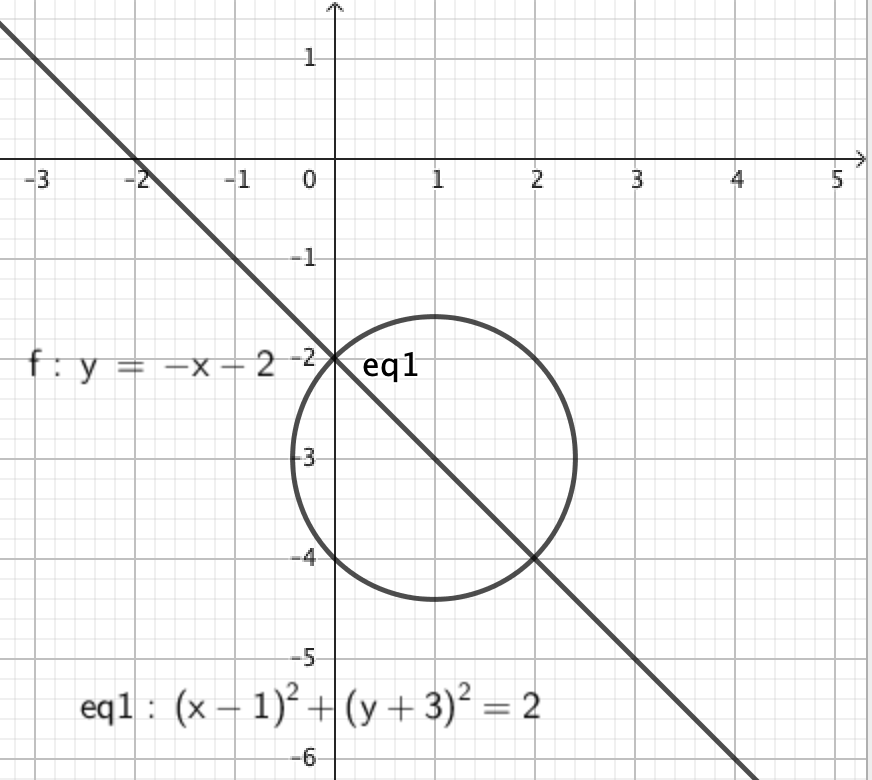
\includegraphics[width=\textwidth]{cirkel.png}
\end{center}
\caption{Cirklen og linjen fra opgaven tegnet i GeoGebra}
\label{fig:cirkel}
\end{figure}
\end{document}
